%%%%%%%%%%%%%%%%%%%%%%%%%%%%%%%%%%%%%%%%%%%%%%%%%%%%%%%%%%%%%%%%
%%%% Please read project_README.md before compiling the code %%%
%%%%%%%%%%%%%%%%%%%%%%%%%%%%%%%%%%%%%%%%%%%%%%%%%%%%%%%%%%%%%%%%

\documentclass{beamer}
\usetheme{Nord}             % import theme

%% import packages %%
\usepackage[utf8]{inputenc}
\usepackage{graphicx}
\usepackage{color}
\usepackage{fontspec}      % font cfg
\usepackage{tabularx}      % tabular cfg
\usepackage{booktabs}      % enable side by side table

%% font setting %%
\setmainfont{Yanone Kaffeesatz}
\setsansfont{Andika New Basic}
\setmonofont{DejaVu Sans Mono}

%% title page content %%
\title{MULTIMODAL SPEECH EMOTION RECOGNITION USING AUDIO AND TEXT}
\subtitle{COMP8240 Group J Project Proposal}
\author{Jan Arvin Lapuz, Alyssa Lim, Le Van Nguyen,\break Ramil Zabala}
\date{September 1, 2020}

\begin{document}
    %% title page %%
    \begin{frame}[plain,noframenumbering]
        \maketitle
    \end{frame}
    
    %% content %%
    \begin{frame}{Overview}
        \begin{itemize}
            \item 2018 IEEE Spoken Language Technology Workshop (SLT)
            \item Rank 14 - Computational Linguistics Category 
                \begin{itemize}
                    \item Google Scholar
                \end{itemize}
            \item Deep Dual Recurrent Encoder Model
            \begin{itemize}
                \item audio signals \& text data
                \item speech data >> signal level >> language level
                \item emotion categories:
                \begin{itemize}
                    \item angry
                    \item happy
                    \item sad
                    \item neutral
                \end{itemize}
                \item accuracy: 68.8\% to 71.8\% (IEMOCAP dataset)
            \end{itemize}
            \item CNN Long Short-Term Memory Neural Networks
                \begin{itemize}
                    \item speech recognition
                    \item natural language processing
                \end{itemize}
        \end{itemize}
    \end{frame}
        
    \begin{frame}{Specifications}
        \begin{description}
            \item[Requirements]
                python 2.7 \\
                nltk 3.3 \\
                scikit-learn 0.20.0 \\
                tensorflow 1.4 \\
                Google ASR system \\
                OpenSMILE toolkit
            \item[Input Features]
                Mel-Frequency Cepstral Coefficients (MFCCs) \\
                Prosodoic Features \\
                Word Tokens \\
        \end{description}
    \end{frame}
    
    \begin{frame}{Specifications}
        \begin{description}
        \item[Source Code]
            https://github.com/david-yoon/multimodal-speech-emotion
        \item[Original Datasets]
                IEMOCAP dataset \\
                ASR system processes IEMOCAP audio data
        \item[New Dataset]
            \begin{itemize}
                \item 25 new data per member
                \item existing dataset from other research of the same topic
            \end{itemize}
        \end{description}
    \end{frame}
    
    \begin{frame}{Model}
        \begin{figure}
            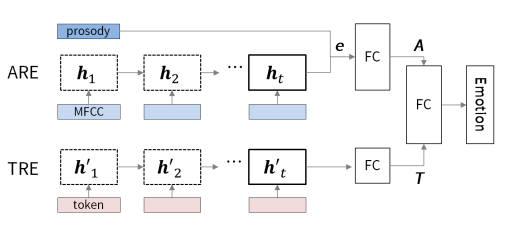
\includegraphics[width = 1\linewidth]{Images/model.PNG}
            \caption{Multimodal Dual Recurrent Encoder (MDRE)}
            \label{fig:MDRE}
        \end{figure}
    \end{frame}
        
    \begin{frame}{Research Results}
        \begin{minipage}{.5\textwidth}
            \centering
            \caption\textcolor{NordGreen}{Multimodal Speech Emotion Recognition Results}
            \begin{tabularx}{.9\linewidth}{l|c}
                \hline
                \textbf{Model} & \textbf{WAP} \\
                \hline
                ARE & $0.546 \pm 0.009$ \\
                TRE & $0.635 \pm 0.018$ \\
                \textcolor{NordGreen}{MDRE} & 
                    $\textcolor{NordGreen}{0.718 \pm 0.019}$ \\
                MDREA & $0.690 \pm 0.019$ \\
                \hline
                TRE-ASR & $0.593 \pm 0.022$ \\
                \textcolor{NordGreen}{MDRE-ASR} & 
                    $\textcolor{NordGreen}{0.691 \pm 0.019}$ \\
                MDREA-ASR & $0.677 \pm 0.013$ \\
                \hline
            \end{tabularx}
        \end{minipage}%
        \begin{minipage}{.5\textwidth}
            \centering
            \caption\textcolor{NordGreen}{Novel Models' Results}
            \begin{tabularx}{.9\linewidth}{l|c}
                \hline
                \textbf{Model} & \textbf{WAP} \\
                \hline
                ACNN & $0.561$ \\
                LLD RNN-attn & $0.635$ \\
                RNN(prop.)-ELM & $0.628$ \\
                \textcolor{NordGreen}{3CNN-LSTM10H} &                              $\textcolor{NordGreen}{0.688}$ \\
                \hline
            \end{tabularx}
        \end{minipage}
    \end{frame}
\end{document}